\subsection{What a repair changes for an investigator}
Figure~\ref{fig:application-example} illustrates both useful recovery and harm in the earlier loan study. In the successful example, the retrieved application history loses an unrelated call and gains its missing offer-creation record. Its recorded cancellations remain visible. The second example shows why aggregate improvement is insufficient: repair removes the only correctly retrieved event of a short offer history while leaving an unrelated event. An investigator would then receive a less faithful account of that offer. These are post hoc illustrations from one original trial, selected by documented rules, not additional independent validation or estimates of how often each outcome occurs.

\begin{figure}[t]
\centering
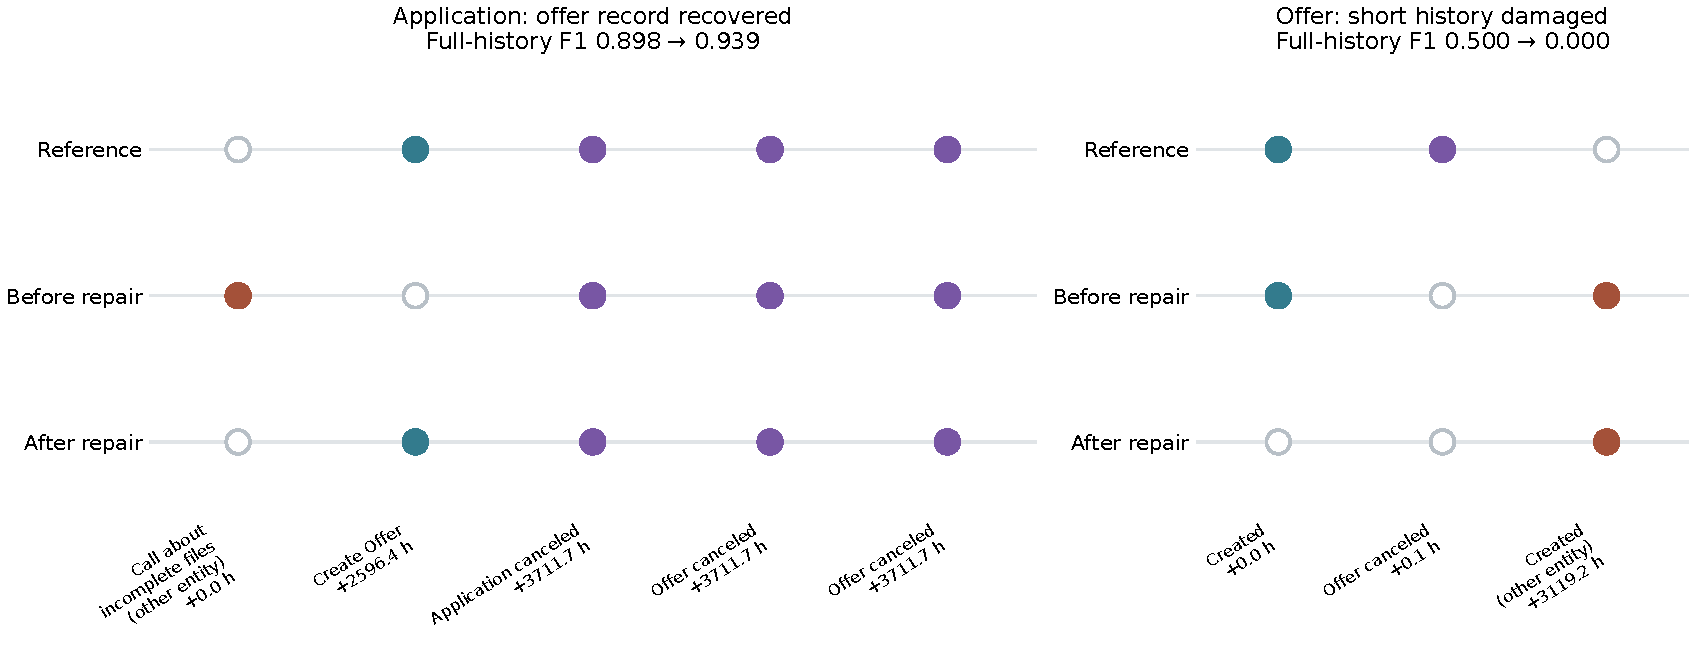
\includegraphics[width=\linewidth]{../../paper/figures/confirmation_loan_cases.pdf}
\caption{Application consequences in the earlier controlled-fault loan experiment. Filled markers denote retrieved records; empty markers denote absent records. Purple marks cancellation evidence, blue other correct records, and brown unrelated records. The left panel shows changed associations and cancellation records from a 26-record reference history; the right shows the full three-record union for a two-record reference history. Displayed F1 scores use complete histories. Columns are chronological but evenly spaced; elapsed hours are labelled.}
\label{fig:application-example}
\end{figure}
